\documentclass[11pt]{report}

% Paquetes y configuraciones adicionales
\usepackage{graphicx}
\usepackage[export]{adjustbox}
\usepackage{caption}
\usepackage{float}
\usepackage{titlesec}
\usepackage{geometry}
\usepackage[hidelinks]{hyperref}
\usepackage{titling}
\usepackage{titlesec}
\usepackage{parskip}
\usepackage{wasysym}
\usepackage{tikzsymbols}
\usepackage{fancyvrb}
\usepackage{xurl}
\usepackage{hyperref}
\usepackage{subcaption}

\usepackage{listings}
\usepackage{xcolor}

\usepackage[spanish]{babel}

\newcommand{\subtitle}[1]{
  \posttitle{
    \par\end{center}
    \begin{center}\large#1\end{center}
    \vskip0.5em}
}

% Configura los márgenes
\geometry{
  left=2cm,   % Ajusta este valor al margen izquierdo deseado
  right=2cm,  % Ajusta este valor al margen derecho deseado
  top=3cm,
  bottom=3cm,
}

% Configuración de los títulos de las secciones
\titlespacing{\section}{0pt}{\parskip}{\parskip}
\titlespacing{\subsection}{0pt}{\parskip}{\parskip}
\titlespacing{\subsubsection}{0pt}{\parskip}{\parskip}

% Redefinir el formato de los capítulos y añadir un punto después del número
\makeatletter
\renewcommand{\@makechapterhead}[1]{%
  \vspace*{0\p@} % Ajusta este valor para el espaciado deseado antes del título del capítulo
  {\parindent \z@ \raggedright \normalfont
    \ifnum \c@secnumdepth >\m@ne
        \huge\bfseries \thechapter.\ % Añade un punto después del número
    \fi
    \interlinepenalty\@M
    #1\par\nobreak
    \vspace{10pt} % Ajusta este valor para el espacio deseado después del título del capítulo
  }}
\makeatother

% Configura para que cada \chapter no comience en una pagina nueva
\makeatletter
\renewcommand\chapter{\@startsection{chapter}{0}{\z@}%
    {-3.5ex \@plus -1ex \@minus -.2ex}%
    {2.3ex \@plus.2ex}%
    {\normalfont\Large\bfseries}}
\makeatother

% Configurar los colores para el código
\definecolor{codegreen}{rgb}{0,0.6,0}
\definecolor{codegray}{rgb}{0.5,0.5,0.5}
\definecolor{codepurple}{rgb}{0.58,0,0.82}
\definecolor{backcolour}{rgb}{0.95,0.95,0.92}

% Configurar el estilo para el código
\lstdefinestyle{mystyle}{
  backgroundcolor=\color{backcolour},   
  commentstyle=\color{codegreen},
  keywordstyle=\color{magenta},
  numberstyle=\tiny\color{codegray},
  stringstyle=\color{codepurple},
  basicstyle=\ttfamily\footnotesize,
  breakatwhitespace=false,         
  breaklines=true,                 
  captionpos=b,                    
  keepspaces=true,                 
  numbers=left,                    
  numbersep=5pt,                  
  showspaces=false,                
  showstringspaces=false,
  showtabs=false,                  
  tabsize=2
}

%==============================================================================
% Cosas para la documentación LateX
% % Sangría
% \setlength{\parindent}{1em}Texto

% % Quitar sangría
% \noindent

% % Punto
% \CIRCLE \ \ \textbf{Texto} \emph{algo}
% \begin{itemize}
%   \item \textbf{Negrita:} Texto
%   \item \textbf{Negrita:} Texto
% \end{itemize}

% % Introducir código
% \begin{center}
%   \begin{BVerbatim}
%     ... Código
%   \end{BVerbatim}
% \end{center}

% Poner una imagen
% \begin{figure}[H]
%   \centering
%   \includegraphics[scale=0.55]{img/}
%   \caption{Exportación de la base de datos en formato sql}
%   \label{fig:exportación de la base de datos en formato sql}
% \end{figure}

% Poner dos imágenes
% \begin{figure}[H]
%   \begin{subfigure}{0.5\textwidth}
%     \centering
%     \includegraphics[scale=0.45]{img/}
%     \caption{Texto imagen 1}
%   \end{subfigure}%
%   \begin{subfigure}{0.5\textwidth}
%     \centering
%     \includegraphics[scale=0.45]{img/}
%     \caption{Texto imagen 2}
%   \end{subfigure}
%   \caption{Texto general}
% \end{figure}

% % Poner una tabla
% \begin{table}[H]
%   \centering
%   \begin{tabular}{|c|c|c|c|}
%     \hline
%     \textbf{Campo 1} & \textbf{Campo 2} & \textbf{Campo 3} & \textbf{Campo 4} \\ \hline
%     Texto & Texto & Texto & Texto \\ \hline
%     Texto & Texto & Texto & Texto \\ \hline
%     Texto & Texto & Texto & Texto \\ \hline
%     Texto & Texto & Texto & Texto \\ \hline
%   \end{tabular}
%   \caption{Nombre de la tabla}
%   \label{tab:nombre de la tabla}
% \end{table}

% % Poner codigo de un lenguaje a partir de un archivo
% \lstset{style=mystyle}
% The next code will be directly imported from a file
% \lstinputlisting[language=Python]{code.py}

% “Texto entre comillas dobles”

%==============================================================================

\begin{document}

% Portada del informe
\title{Práctica 07: Diseño y simplificación de gramáticas}
\subtitle{Computabilidad y Algoritmia}
\author{Cheuk Kelly Ng Pante (alu0101364544@ull.edu.es)}
\date{29/10/2024}

\maketitle

\pagestyle{empty} % Desactiva la numeración de página para el índice

% Índice
\tableofcontents

% Nueva página
\cleardoublepage

\pagestyle{plain} % Vuelve a activar la numeración de página
\setcounter{page}{1} % Reinicia el contador de página a 1

% Se pide para cada ejercicio:
% 1. El enunciado del ejercicio.
% 2. Una breve explicacion de la gramatica diseñada, describiendo los criterios se-
% guidos durante el dise ̃no, as ́ı como las reglas y elementos que la componen.
% 3. Una imagen con la gram ́atica dise ̃nada en JFLAP.
% 4. Al menos tres ejemplos de cadenas que pueden ser generadas a partir de la
% gram ́atica (incluir cada  ́arbol de an ́alisis sint ́actico).
% 5. Una descripci ́on detallada del proceso, paso a paso, de simplificaci ́on de la
% gram ́atica junto con una verificaci ́on de que el resultado realizado de forma
% aut ́onoma coincide con el resultado obtenido con cada algoritmo en JFLAP

% Secciones del informe
% Capitulo 1
\chapter{Ejercicios de diseño de gramáticas}
% Ejericio 1
\section{Diseñar una gramática independiente del contexto que genere el lenguaje \texorpdfstring{$L = \{a^n b^n \mid n \geq 0\}$}{L = \{a^n b^n | n >= 0\}}}
\begin{itemize}
  \item \textbf{Explicación de la gramática:} El lenguaje $L = \{a^n b^n \mid n \geq 0\}$ acepta todas las cadenas que tienen el mismo número de símbolos de
  a's seguidos por el mismo número de b's. La gramática diseñada para el lenguaje $L$ sigue la siguiente estructura:
  \begin{itemize}
    \item $S \rightarrow aSb \mid \varepsilon$
  \end{itemize}
  \item \textbf{Imagen de la gramática en JFLAP:} La gramática diseñada en JFLAP se muestra en la siguiente figura:
  \begin{figure}[H]
    \centering
    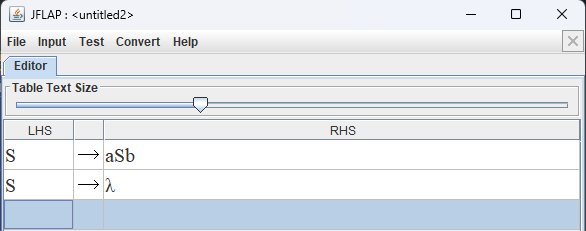
\includegraphics[scale=0.55]{img/grammar_01.png}
    \caption{Gramática diseñada en JFLAP para el lenguaje $L = \{a^n b^n \mid n \geq 0\}$}
  \end{figure}
  \item \textbf{Ejemplos de cadenas generadas:}
  \begin{itemize}
    \item \textbf{Cadena 1:} $aabb$
    \begin{itemize}
      \item \textbf{Árbol de análisis sintáctico:} El árbol de análisis sintáctico para la cadena $aabb$ se muestra en la siguiente figura:
      \begin{figure}[H]
        \centering
        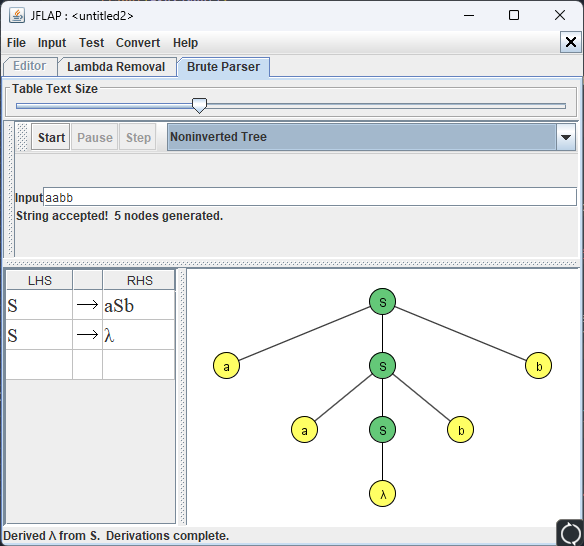
\includegraphics[scale=0.5]{img/grammar_01_tree_1.png}
        \caption{Árbol de análisis sintáctico para la cadena $aabb$}
        \label{fig:arbol1}
      \end{figure}
    \end{itemize}
    \item \textbf{Cadena 2:} $aaabbb$
    \begin{itemize}
      \item \textbf{Árbol de análisis sintáctico:} El árbol de análisis sintáctico para la cadena $aaabbb$ se muestra en la siguiente figura:
      \begin{figure}[H]
        \centering
        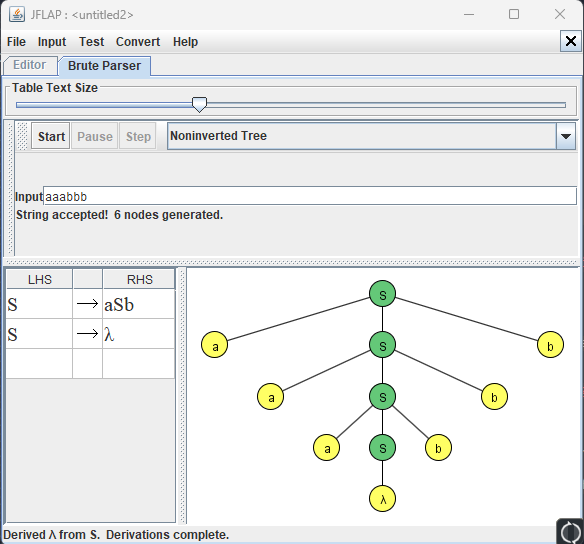
\includegraphics[scale=0.5]{img/grammar_01_tree_2.png}
        \caption{Árbol de análisis sintáctico para la cadena $aaabbb$}
        \label{fig:arbol2}
      \end{figure}
    \end{itemize}
    \item \textbf{Cadena 3:} $aaaaaabbbbbb$
    \begin{itemize}
      \item \textbf{Árbol de análisis sintáctico:} El árbol de análisis sintáctico para la cadena $aaaaaabbbbbb$ se muestra en la siguiente figura:
      \begin{figure}[H]
        \centering
        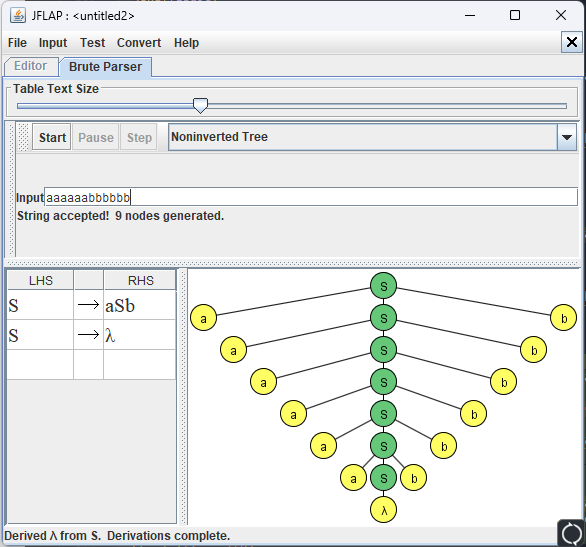
\includegraphics[scale=0.5]{img/grammar_01_tree_3.png}
        \caption{Árbol de análisis sintáctico para la cadena $aaaaaabbbbbb$}
        \label{fig:arbol3}
      \end{figure}
    \end{itemize}
  \end{itemize}
  \item \textbf{Imagen de la gramática simplificada en JFLAP:} La gramática simplificada en JFLAP se muestra en la siguiente figura:
  \begin{figure}[H]
    \centering
    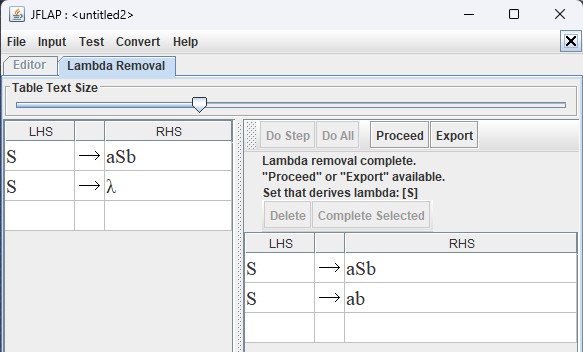
\includegraphics[scale=0.55]{img/grammar_01_simplified.png}
    \caption{Gramática simplificada en JFLAP para el lenguaje $L = \{a^n b^n \mid n \geq 0\}$}
    \label{fig:gramatica1_simplified}
  \end{figure}
\end{itemize}

\newpage

% Ejericio 2
\section{Diseñar una gramática independiente del contexto que genere el lenguaje \texorpdfstring{$L = \{a^n b^m \mid n, m \geq 0, n \neq m\}$}{L = \{a^n b^m | n, m >= 0, n ≠ m\}}}
\begin{itemize}
  \item \textbf{Explicación de la gramática:}  El lenguaje $L = \{a^n b^m \mid n, m \geq 0, n \neq m\}$ acepta todas las cadenas de a's seguidas de b's donde el número de a's es diferente del número de b's. Entonces se puede
  dividir en dos casos:
  \begin{itemize}
    \item $n > m$: En este caso, el número de a's es mayor que el número de b's.
    \item $n < m$: En este caso, el número de a's es menor que el número de b's.
  \end{itemize} 
  La gramática diseñada para el lenguaje $L$ sigue la siguiente estructura:
  \begin{itemize}
    \item $S \rightarrow aSb \mid A \mid B$
    \item $A \rightarrow aA \mid a$
    \item $B \rightarrow bB \mid b$
  \end{itemize}
  \item \textbf{Imagen de la gramática en JFLAP:} La gramática diseñada en JFLAP se muestra en la siguiente figura:
  \begin{figure}[H]
    \centering
    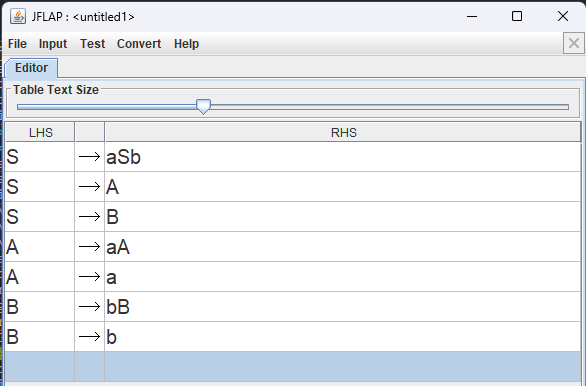
\includegraphics[scale=0.55]{img/grammar_02.png}
    \caption{Gramática diseñada en JFLAP para el lenguaje $L = \{a^n b^m \mid n, m \geq 0, n \neq m\}$}
  \end{figure}

  \newpage

  \item \textbf{Ejemplos de cadenas generadas:}
  \begin{itemize}
    \item \textbf{Cadena 1:} $aab$
    \begin{itemize}
      \item \textbf{Árbol de análisis sintáctico:} El árbol de análisis sintáctico para la cadena $aab$ se muestra en la siguiente figura:
      \begin{figure}[H]
        \centering
        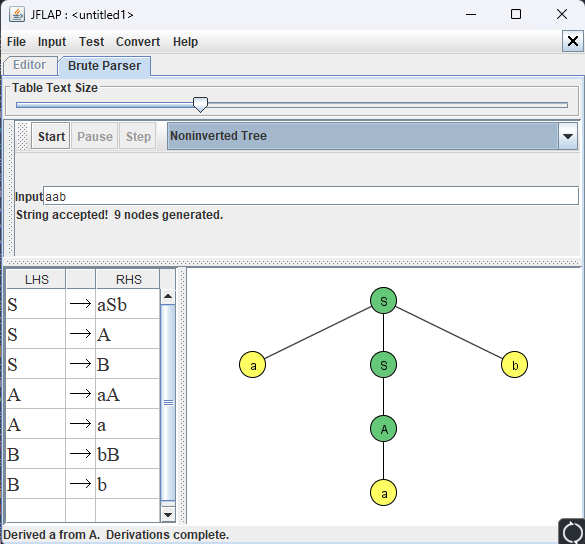
\includegraphics[scale=0.5]{img/grammar_02_tree_1.png}
        \caption{Árbol de análisis sintáctico para la cadena $aab$}
        \label{fig:arbol4}
      \end{figure}
    \end{itemize}
    \item \textbf{Cadena 2:} $abbb$
    \begin{itemize}
      \item \textbf{Árbol de análisis sintáctico:} El árbol de análisis sintáctico para la cadena $abbb$ se muestra en la siguiente figura:
      \begin{figure}[H]
        \centering
        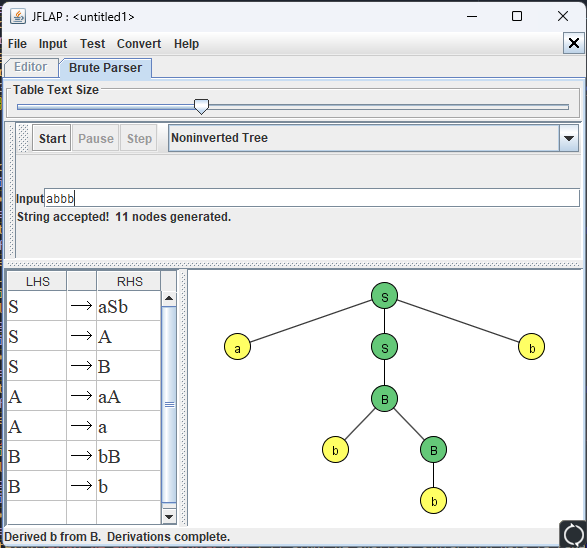
\includegraphics[scale=0.5]{img/grammar_02_tree_2.png}
        \caption{Árbol de análisis sintáctico para la cadena $abbb$}
        \label{fig:arbol5}
      \end{figure}
    \end{itemize}
    \item \textbf{Cadena 3:} $aaaaaaab$
    \begin{itemize}
      \item \textbf{Árbol de análisis sintáctico:} El árbol de análisis sintáctico para la cadena $aaaaaaab$ se muestra en la siguiente figura:
      \begin{figure}[H]
        \centering
        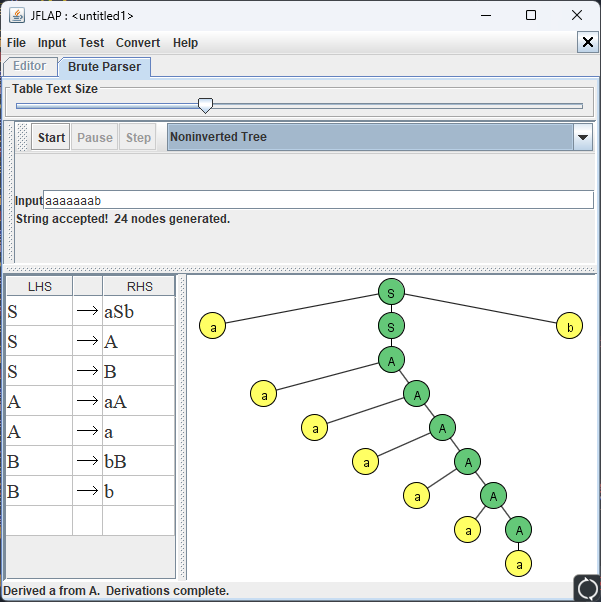
\includegraphics[scale=0.44]{img/grammar_02_tree_3.png}
        \caption{Árbol de análisis sintáctico para la cadena $aaaaaaab$}
        \label{fig:arbol6}
      \end{figure}
    \end{itemize}
  \end{itemize}
  \item \textbf{Imagen de la gramática simplificada en JFLAP:} La gramática simplificada en JFLAP se muestra en la siguiente figura:

  \begin{figure}[H]
    \begin{subfigure}{0.5\textwidth}
      \centering
      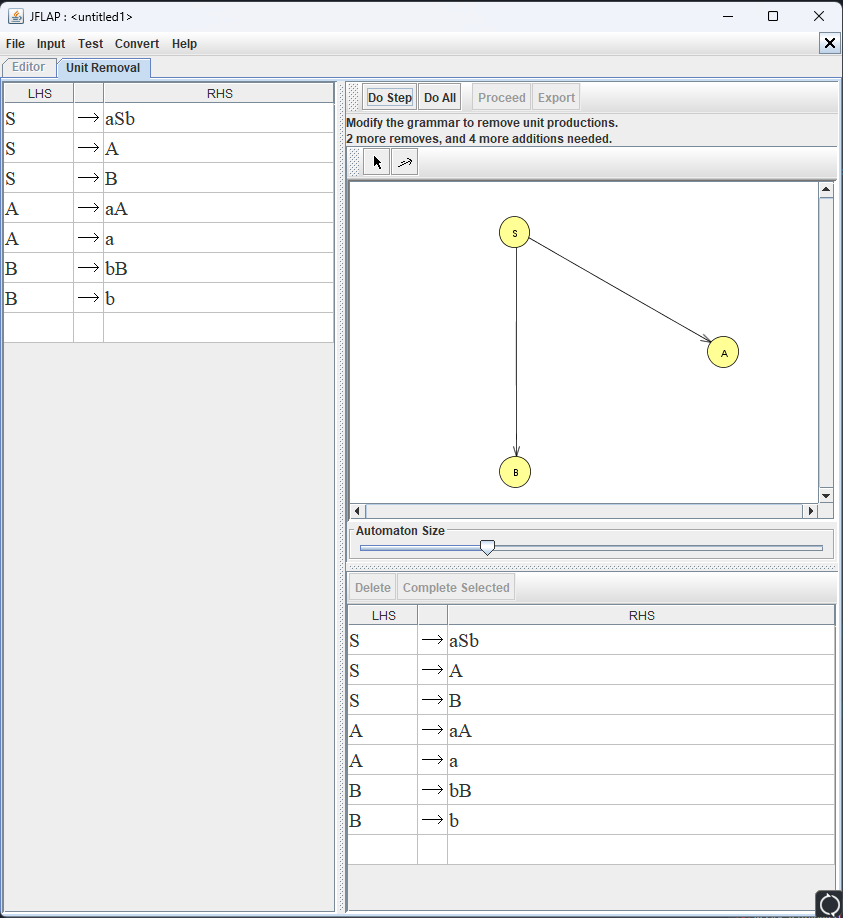
\includegraphics[scale=0.35]{img/grammar_02_simplified_remove_unit_productions.png}
      \caption{Eliminación de producciones unitarias}
    \end{subfigure}%
    \begin{subfigure}{0.5\textwidth}
      \centering
      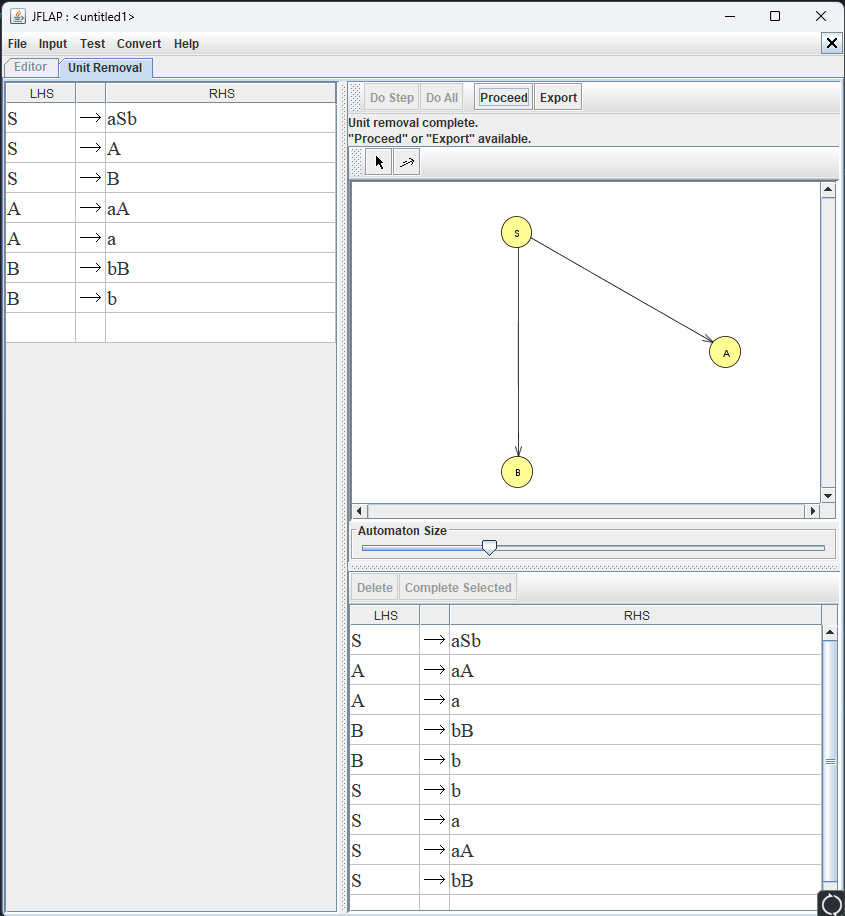
\includegraphics[scale=0.35]{img/grammar_02_simplified.png}
      \caption{Gramática simplificada}
    \end{subfigure}
    \caption{Gramática simplificada en JFLAP para el lenguaje $L = \{a^n b^m \mid n, m \geq 0, n \neq m\}$}
  \end{figure}
\end{itemize}

\newpage

% Ejericio 3
\section{Diseñar una gramática independiente del contexto que genere el lenguaje \texorpdfstring{$L = \{ww^I \mid w \in \{a, b\}^*\}$}{L = \{ww^I | w ∈ \{a, b\}^*\}}}
\begin{itemize}
  \item \textbf{Explicación de la gramática:} El lenguaje $L = \{ww^I \mid w \in \{a, b\}^*\}$ acepta todas las cadenas que son palíndromas sobre el alfabeto $\Sigma = \{a, b\}$. La gramática diseñada para el lenguaje $L$ sigue la siguiente estructura:
  \begin{itemize}
    \item $S \rightarrow aSa \mid bSb \mid \varepsilon$
  \end{itemize}
  \item \textbf{Imagen de la gramática en JFLAP:} La gramática diseñada en JFLAP se muestra en la siguiente figura:
  \begin{figure}[H]
    \centering
    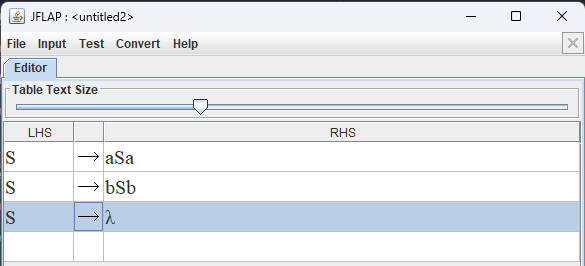
\includegraphics[scale=0.55]{img/grammar_03.png}
    \caption{Gramática diseñada en JFLAP para el lenguaje $L = \{ww^I \mid w \in \{a, b\}^*\}$}
  \end{figure}
  \item \textbf{Ejemplos de cadenas generadas:}
  \begin{itemize}
    \item \textbf{Cadena 1:} $aa$
    \begin{itemize}
      \item \textbf{Árbol de análisis sintáctico:} El árbol de análisis sintáctico para la cadena $aa$ se muestra en la siguiente figura:
      \begin{figure}[H]
        \centering
        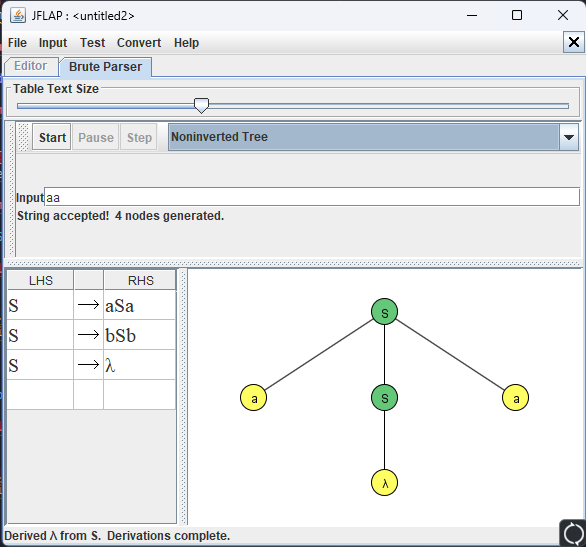
\includegraphics[scale=0.5]{img/grammar_03_tree_1.png}
        \caption{Árbol de análisis sintáctico para la cadena $aa$}
        \label{fig:arbol7}
      \end{figure}
    \end{itemize}
    \item \textbf{Cadena 2:} $abba$
    \begin{itemize}
      \item \textbf{Árbol de análisis sintáctico:} El árbol de análisis sintáctico para la cadena $abba$ se muestra en la siguiente figura:
      \begin{figure}[H]
        \centering
        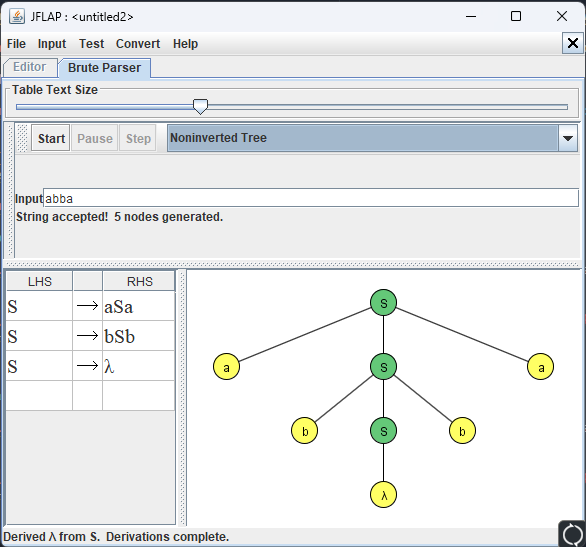
\includegraphics[scale=0.5]{img/grammar_03_tree_2.png}
        \caption{Árbol de análisis sintáctico para la cadena $abba$}
        \label{fig:arbol8}
      \end{figure}
    \end{itemize}
    \item \textbf{Cadena 3:} $abbaabba$
    \item \textbf{Árbol de análisis sintáctico:} El árbol de análisis sintáctico para la cadena $abbaabba$ se muestra en la siguiente figura:
    \begin{figure}[H]
      \centering
      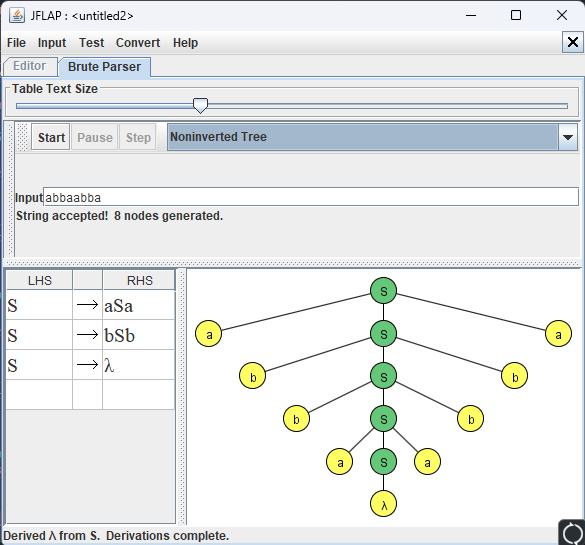
\includegraphics[scale=0.5]{img/grammar_03_tree_3.png}
      \caption{Árbol de análisis sintáctico para la cadena $abbaabba$}
      \label{fig:arbol9}
    \end{figure}
  \end{itemize}
  \item \textbf{Imagen de la gramática simplificada en JFLAP:} La gramática simplificada en JFLAP se muestra en la siguiente figura:
  \begin{figure}[H]
    \centering
    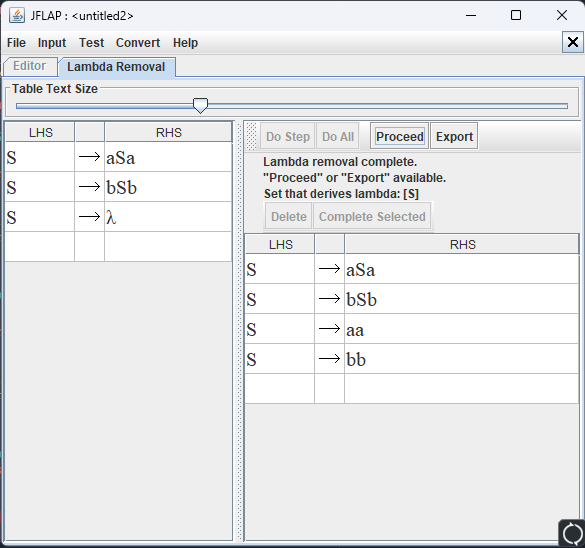
\includegraphics[scale=0.55]{img/grammar_03_simplified.png}
    \caption{Gramática simplificada en JFLAP para el lenguaje $L = \{ww^I \mid w \in \{a, b\}^*\}$}
    \label{fig:gramatica3_simplified}
  \end{figure}
\end{itemize}

\newpage

% Ejericio 4
\section{Diseñar una gramática independiente del contexto que genere el lenguaje $L = \{a^n b^m c^n \mid n \geq 0, m \ impar\}$}
\begin{itemize}
  \item \textbf{Explicación de la gramática:} El lenguaje $L = \{a^n b^m c^n \mid n \geq 0, m \ impar\}$ acepta todas las cadenas que empiezan con una cantidad $n$ de símbolos $a$, luego tienen una cantidad $m$ de símbolos $b$, y terminan con una cantidad 
  $n$ de símbolos $c$. La gramática diseñada para el lenguaje $L$ sigue la siguiente estructura:
  \begin{itemize}
    \item $S \rightarrow aSc \mid A$
    \item $A \rightarrow bAb \mid b$
  \end{itemize}
  \item \textbf{Imagen de la gramática en JFLAP:} La gramática diseñada en JFLAP se muestra en la siguiente figura:
  \begin{figure}[H]
    \centering
    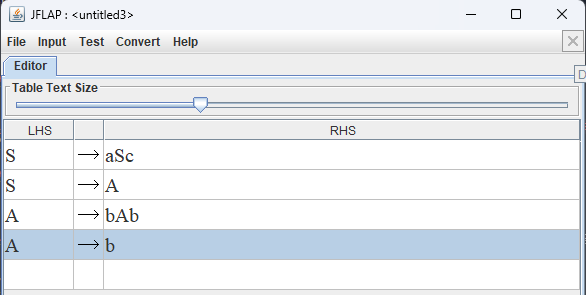
\includegraphics[scale=0.5]{img/grammar_04.png}
    \caption{Gramática diseñada en JFLAP para el lenguaje $L = \{a^n b^m c^n \mid n \geq 0, m \ impar\}$}
  \end{figure}
  \item \textbf{Ejemplos de cadenas generadas:}
  \begin{itemize}
    \item \textbf{Cadena 1:} $b$
    \begin{itemize}
      \item \textbf{Árbol de análisis sintáctico:} El árbol de análisis sintáctico para la cadena $b$ se muestra en la siguiente figura:
      \begin{figure}[H]
        \centering
        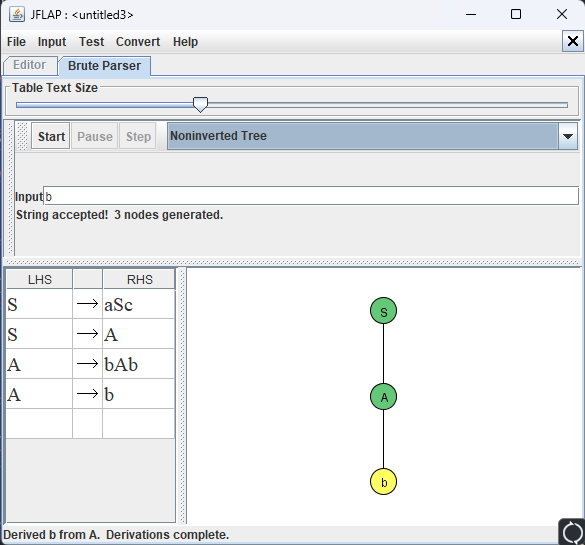
\includegraphics[scale=0.45]{img/grammar_04_tree_1.png}
        \caption{Árbol de análisis sintáctico para la cadena $b$}
        \label{fig:arbol10}
      \end{figure}
    \end{itemize}

    \newpage

    \item \textbf{Cadena 2:} $abc$
    \begin{itemize}
      \item \textbf{Árbol de análisis sintáctico:} El árbol de análisis sintáctico para la cadena $abc$ se muestra en la siguiente figura:
      \begin{figure}[H]
        \centering
        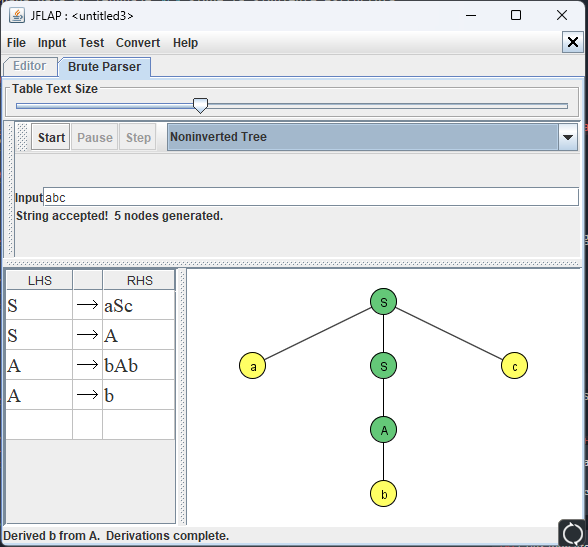
\includegraphics[scale=0.5]{img/grammar_04_tree_2.png}
        \caption{Árbol de análisis sintáctico para la cadena $abc$}
        \label{fig:arbol11}
      \end{figure}
    \end{itemize}
    \item \textbf{Cadena 3:} $aaaabbbcccc$
    \begin{itemize}
      \item \textbf{Árbol de análisis sintáctico:} El árbol de análisis sintáctico para la cadena $aaaabbbcccc$ se muestra en la siguiente figura:
      \begin{figure}[H]
        \centering
        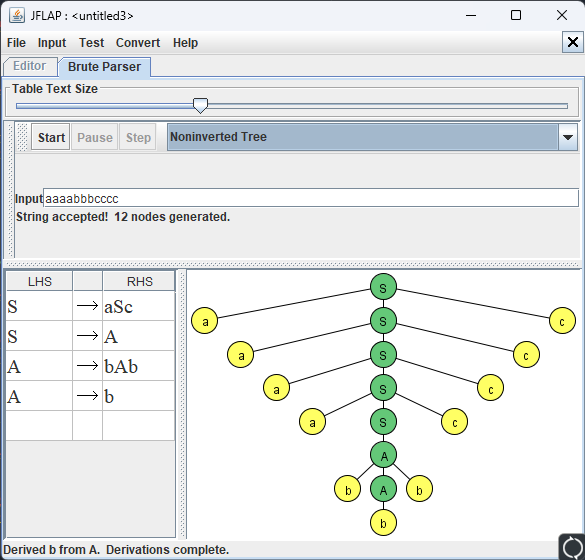
\includegraphics[scale=0.5]{img/grammar_04_tree_3.png}
        \caption{Árbol de análisis sintáctico para la cadena $aaaabbbcccc$}
        \label{fig:arbol12}
      \end{figure}
    \end{itemize}
  \end{itemize}
  \item \textbf{Imagen de la gramática simplificada en JFLAP:} La gramática simplificada en JFLAP se muestra en la siguiente figura:
  \begin{figure}[H]
    \begin{subfigure}{0.5\textwidth}
      \centering
      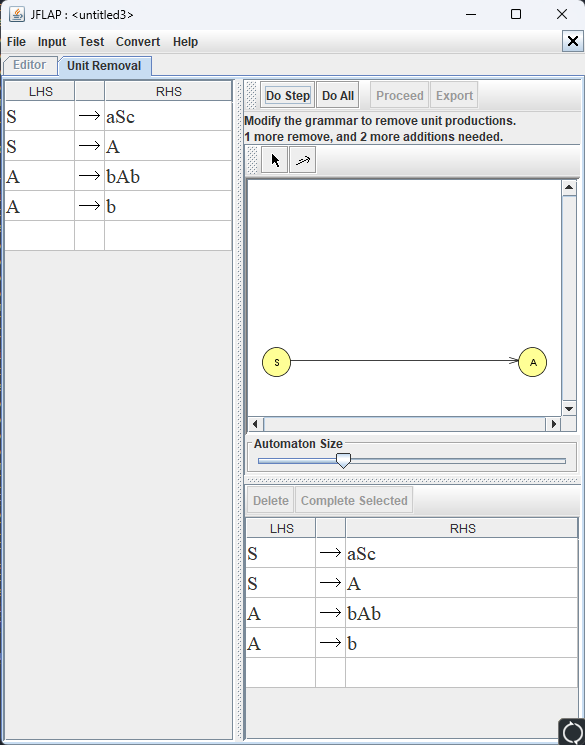
\includegraphics[scale=0.45]{img/grammar_04_simplified_remove_unit_productions.png}
      \caption{Eliminación de producciones unitarias}
    \end{subfigure}%
    \begin{subfigure}{0.5\textwidth}
      \centering
      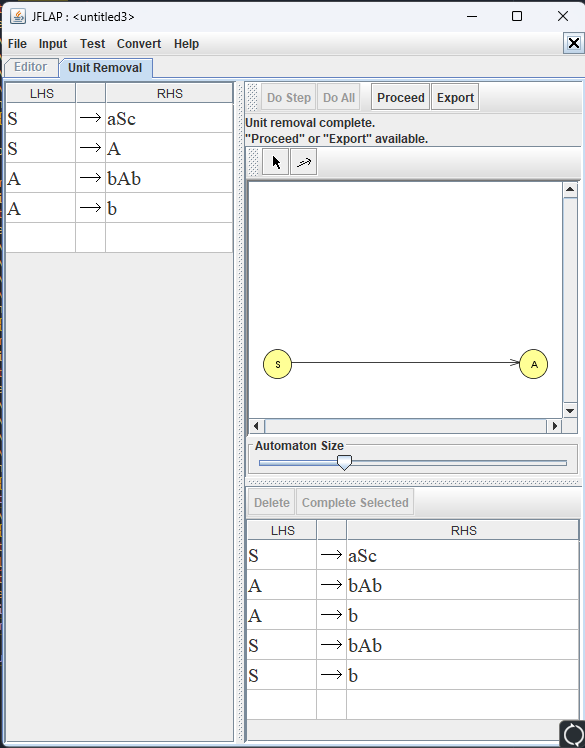
\includegraphics[scale=0.45]{img/grammar_04_simplified.png}
      \caption{Gramática simplificada}
    \end{subfigure}
    \caption{Gramática simplificada en JFLAP para el lenguaje $L = \{a^n b^m \mid n, m \geq 0, n \neq m\}$}
  \end{figure}
\end{itemize}

\newpage

% Ejericio 5
\section{Diseñar una gramática independiente del contexto que genere el lenguaje \texorpdfstring{$L = \{a^n b^m c^m d^n \mid n, m \geq 1\}$}{L = \{a^n b^m c^m d^n | n, m ≥ 1\}}}
\begin{itemize}
  \item \textbf{Explicación de la gramática:} El lenguaje $L = \{a^n b^m c^m d^n \mid n, m \geq 1\}$ acepta todas las cadenas que empiezan con una cantidad $n$ de símbolos $a$, seguido de una cantidad $m$ de símbolos $b$, luego una cantidad $m$ de símbolos $c$, y terminan con una cantidad $n$ de símbolos $d$. La gramática diseñada para el lenguaje $L$ sigue la siguiente estructura:
  \begin{itemize}
    \item $S \rightarrow aSd \mid A$
    \item $A \rightarrow bAc \mid bc$
  \end{itemize}
  \item \textbf{Imagen de la gramática en JFLAP:} La gramática diseñada en JFLAP se muestra en la siguiente figura:
  \begin{figure}[H]
    \centering
    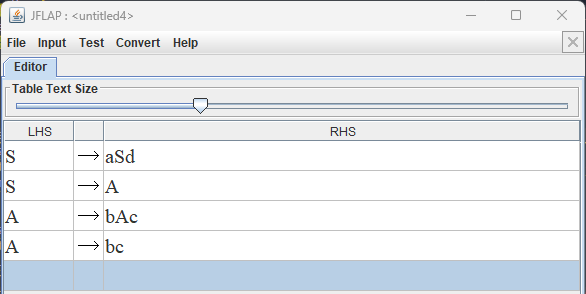
\includegraphics[scale=0.5]{img/grammar_05.png}
    \caption{Gramática diseñada en JFLAP para el lenguaje $L = \{a^n b^m c^m d^n \mid n, m \geq 1\}$}
  \end{figure}
  \item \textbf{Ejemplos de cadenas generadas:}
  \begin{itemize}
    \item \textbf{Cadena 1:} $abcd$
    \begin{itemize}
      \item \textbf{Árbol de análisis sintáctico:} El árbol de análisis sintáctico para la cadena $abcd$ se muestra en la siguiente figura:
      \begin{figure}[H]
        \centering
        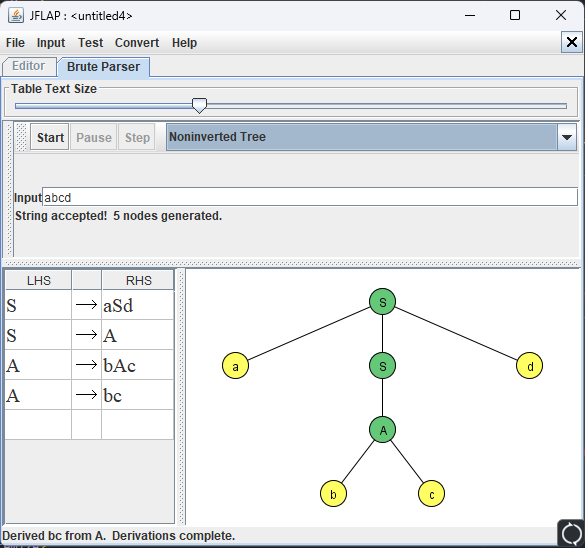
\includegraphics[scale=0.45]{img/grammar_05_tree_1.png}
        \caption{Árbol de análisis sintáctico para la cadena $abcd$}
        \label{fig:arbol13}
      \end{figure}
    \end{itemize}
    \item \textbf{Cadena 2:} $aabbccdd$
    \begin{itemize}
      \item \textbf{Árbol de análisis sintáctico:} El árbol de análisis sintáctico para la cadena $aabbccdd$ se muestra en la siguiente figura:
      \begin{figure}[H]
        \centering
        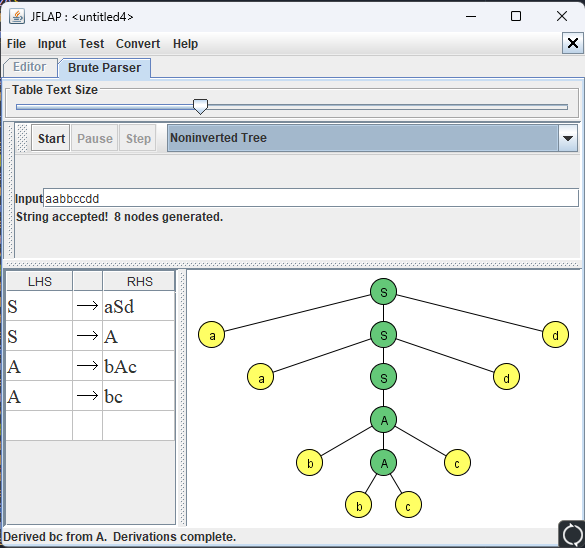
\includegraphics[scale=0.5]{img/grammar_05_tree_2.png}
        \caption{Árbol de análisis sintáctico para la cadena $aabbccdd$}
        \label{fig:arbol14}
      \end{figure}
    \end{itemize}
    \item \textbf{Cadena 3:} $abbbcccd$
    \begin{itemize}
      \item \textbf{Árbol de análisis sintáctico:} El árbol de análisis sintáctico para la cadena $abbbcccd$ se muestra en la siguiente figura:
      \begin{figure}[H]
        \centering
        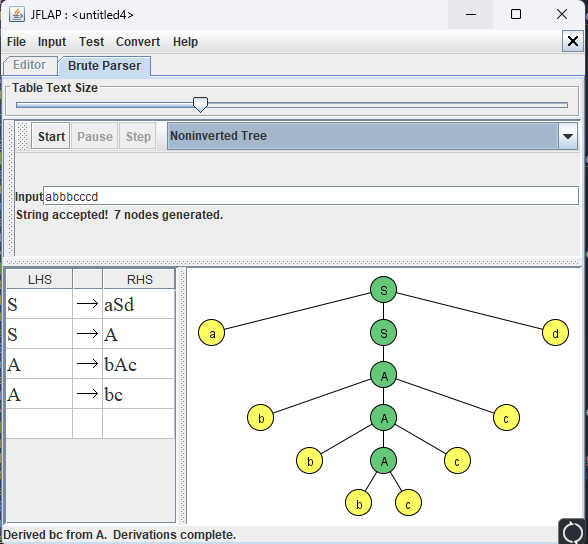
\includegraphics[scale=0.5]{img/grammar_05_tree_3.png}
        \caption{Árbol de análisis sintáctico para la cadena $abbbcccd$}
        \label{fig:arbol15}
      \end{figure}
    \end{itemize}
  \end{itemize}
  \item \textbf{Imagen de la gramática simplificada en JFLAP:} La gramática simplificada en JFLAP se muestra en la siguiente figura:
  \begin{figure}[H]
    \begin{subfigure}{0.5\textwidth}
      \centering
      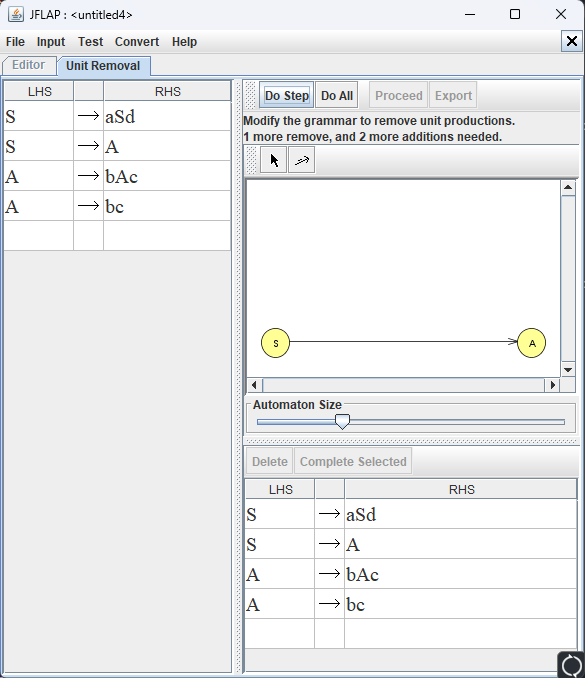
\includegraphics[scale=0.5]{img/grammar_05_simplified_remove_unit_productions.png}
      \caption{Eliminación de producciones unitarias}
    \end{subfigure}%
    \begin{subfigure}{0.5\textwidth}
      \centering
      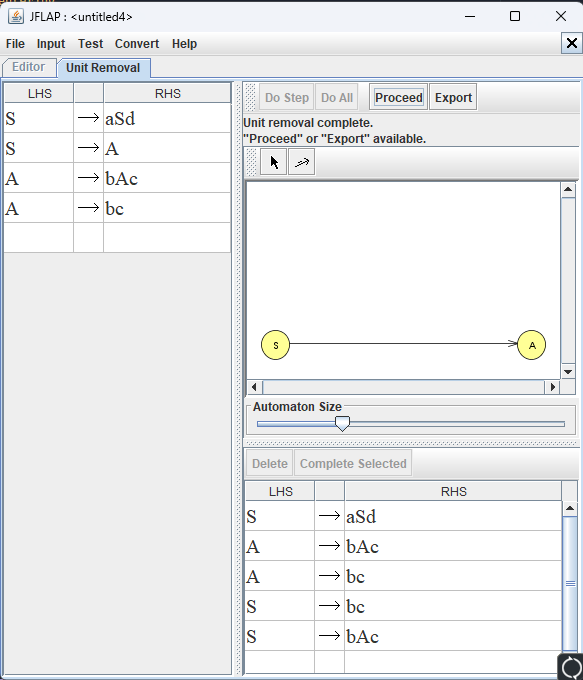
\includegraphics[scale=0.5]{img/grammar_05_simplified.png}
      \caption{Gramática simplificada}
    \end{subfigure}
    \caption{Gramática simplificada en JFLAP para el lenguaje $L = \{a^n b^m c^m d^n \mid n, m \geq 1\}$}
  \end{figure}
\end{itemize}

\newpage

% Ejericio 6
\section{Diseñar una gramática independiente del contexto que genere el lenguaje \texorpdfstring{$L = \{a^n b^m \mid n > m \geq 0\}$}{L = \{a^n b^m | n > m ≥ 0\}}}
\begin{itemize}
  \item \textbf{Explicación de la gramática:} El lenguaje $L = \{a^n b^m \mid n > m \geq 0\}$ acepta todas las cadenas que tienen más símbolos de a's que de b's. La gramática diseñada para el lenguaje $L$ sigue la siguiente estructura:
  \begin{itemize}
    \item $S \rightarrow aS \mid aSb \mid \varepsilon$
  \end{itemize}
  \item \textbf{Imagen de la gramática en JFLAP:} La gramática diseñada en JFLAP se muestra en la siguiente figura:
  \begin{figure}[H]
    \centering
    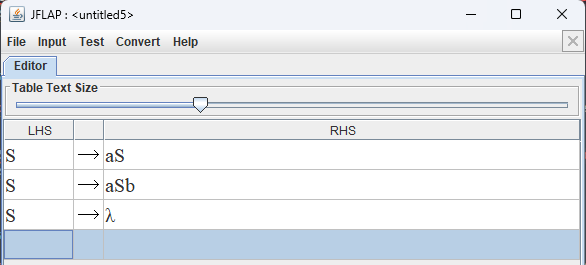
\includegraphics[scale=0.5]{img/grammar_06.png}
    \caption{Gramática diseñada en JFLAP para el lenguaje $L = \{a^n b^m \mid n > m \geq 0\}$}
  \end{figure}
  \item \textbf{Ejemplos de cadenas generadas:}
  \begin{itemize}
    \item \textbf{Cadena 1:} $aab$
    \begin{itemize}
      \item \textbf{Árbol de análisis sintáctico:} El árbol de análisis sintáctico para la cadena $aab$ se muestra en la siguiente figura:
      \begin{figure}[H]
        \centering
        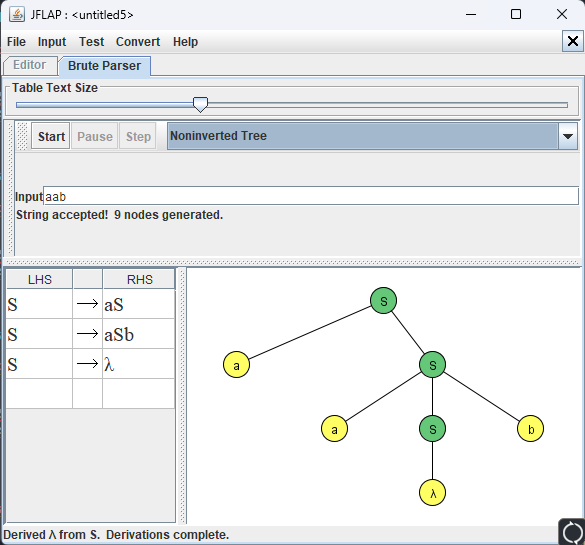
\includegraphics[scale=0.5]{img/grammar_06_tree_1.png}
        \caption{Árbol de análisis sintáctico para la cadena $aab$}
        \label{fig:arbol16}
      \end{figure}
    \end{itemize}
    \item \textbf{Cadena 2:} $aaaaabbb$
    \begin{itemize}
      \item \textbf{Árbol de análisis sintáctico:} El árbol de análisis sintáctico para la cadena $aaaaabbb$ se muestra en la siguiente figura:
      \begin{figure}[H]
        \centering
        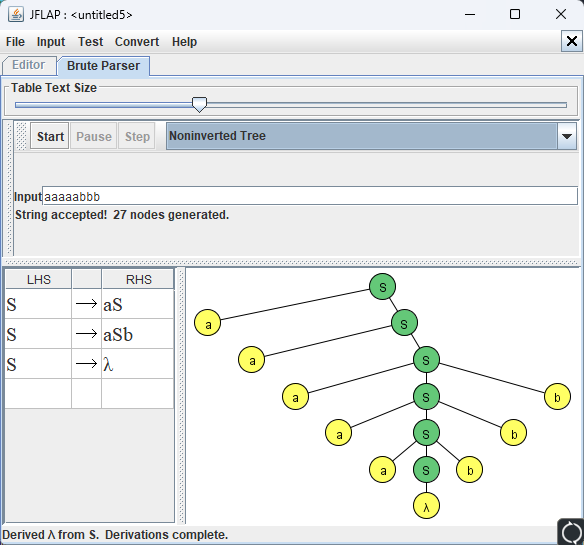
\includegraphics[scale=0.5]{img/grammar_06_tree_2.png}
        \caption{Árbol de análisis sintáctico para la cadena $aaaaabbb$}
        \label{fig:arbol17}
      \end{figure}
    \end{itemize}
    \item \textbf{Cadena 3:} $aaaaaaabbbbb$
    \begin{itemize}
      \item \textbf{Árbol de análisis sintáctico:} El árbol de análisis sintáctico para la cadena $aaaaaaabbbbb$ se muestra en la siguiente figura:
      \begin{figure}[H]
        \centering
        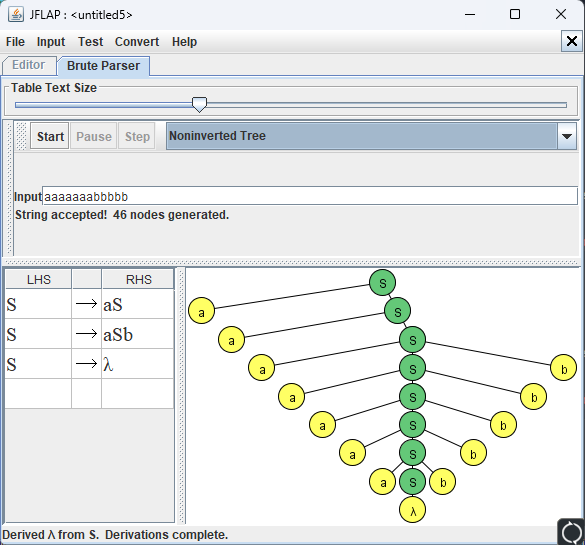
\includegraphics[scale=0.5]{img/grammar_06_tree_3.png}
        \caption{Árbol de análisis sintáctico para la cadena $aaaaaaabbbbb$}
        \label{fig:arbol18}
      \end{figure}
    \end{itemize}
  \end{itemize}
  \item \textbf{Imagen de la gramática simplificada en JFLAP:} La gramática simplificada en JFLAP se muestra en la siguiente figura:
  \begin{figure}[H]
    \centering
    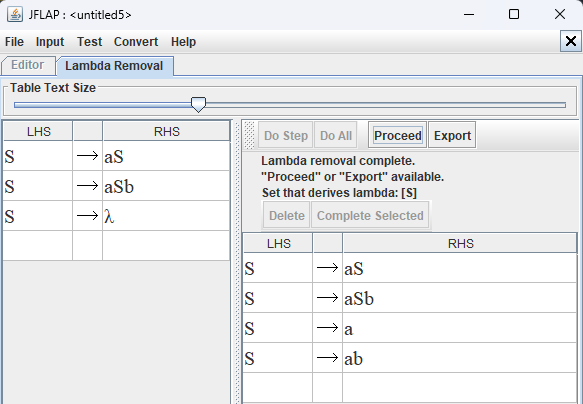
\includegraphics[scale=0.6]{img/grammar_06_simplified.png}
    \caption{Gramática simplificada en JFLAP para el lenguaje $L = \{a^n b^m \mid n > m \geq 0\}$}
    \label{fig:gramatica6_simplified}
  \end{figure}
\end{itemize}

\newpage

% Ejericio 7
\section{Diseñar una gramática independiente del contexto que genere el lenguaje $L = \{a^i b^j c^{i+j} \mid i, \ j \geq 1, \ i + j \ par\}$}
\begin{itemize}
  \item \textbf{Explicación de la gramática:} El lenguaje $L = \{a^i b^j c^{i+j} \mid i, \ j \geq 1, \ i + j \ par\}$ acepta todas las cadenas que tienen una cantidad $i$ de a's, seguido de una cantidad $j$ de b's, y terminan con una cantidad $i + j$ de c's, donde la suma de $i$ y $j$ es un número par. La gramática diseñada para el lenguaje $L$ sigue la siguiente estructura:
  \begin{itemize}
    \item $S \rightarrow aSc \mid A$
    \item $A \rightarrow bAc \mid bc$
  \end{itemize}
  \item \textbf{Imagen de la gramática en JFLAP:} La gramática diseñada en JFLAP se muestra en la siguiente figura:
  \begin{figure}[H]
    \centering
    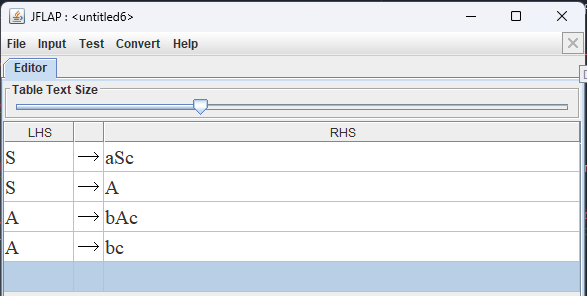
\includegraphics[scale=0.5]{img/grammar_07.png}
    \caption{Gramática diseñada en JFLAP para el lenguaje $L = \{a^i b^j c^{i+j} \mid i, \ j \geq 1, \ i + j \ par\}$}
  \end{figure}
  \item \textbf{Ejemplos de cadenas generadas:}
  \begin{itemize}
    \item \textbf{Cadena 1:} $abcc$
    \begin{itemize}
      \item \textbf{Árbol de análisis sintáctico:} El árbol de análisis sintáctico para la cadena $abcc$ se muestra en la siguiente figura:
      \begin{figure}[H]
        \centering
        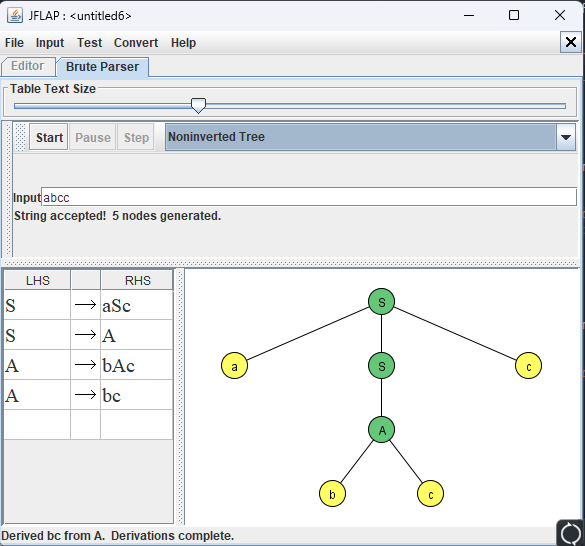
\includegraphics[scale=0.45]{img/grammar_07_tree_1.png}
        \caption{Árbol de análisis sintáctico para la cadena $abcc$}
        \label{fig:arbol19}
      \end{figure}
    \end{itemize}
    \item \textbf{Cadena 2:} $aabbcccc$
    \begin{itemize}
      \item \textbf{Árbol de análisis sintáctico:} El árbol de análisis sintáctico para la cadena $aabbcccc$ se muestra en la siguiente figura:
      \begin{figure}[H]
        \centering
        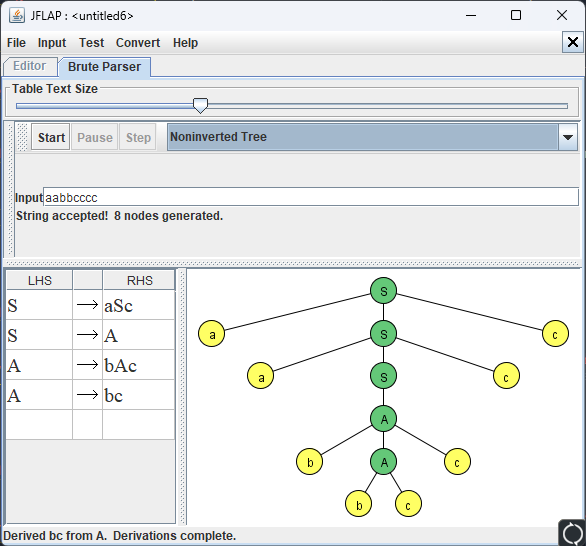
\includegraphics[scale=0.5]{img/grammar_07_tree_2.png}
        \caption{Árbol de análisis sintáctico para la cadena $aabbcccc$}
        \label{fig:arbol20}
      \end{figure}
    \end{itemize}
    \item \textbf{Cadena 3:} $abbbcccc$
    \begin{itemize}
      \item \textbf{Árbol de análisis sintáctico:} El árbol de análisis sintáctico para la cadena $abbbcccc$ se muestra en la siguiente figura:
      \begin{figure}[H]
        \centering
        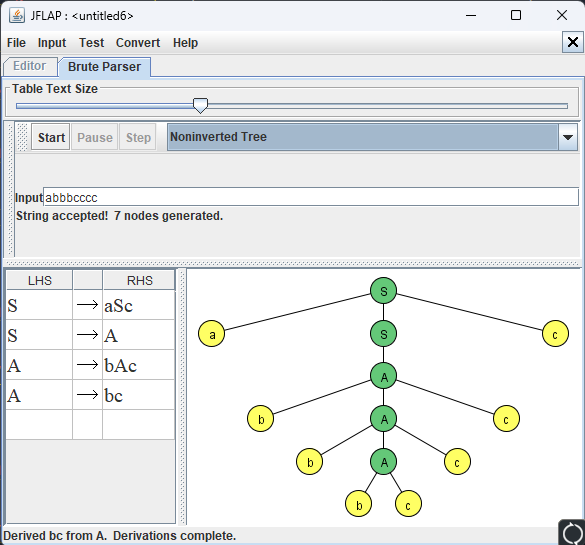
\includegraphics[scale=0.5]{img/grammar_07_tree_3.png}
        \caption{Árbol de análisis sintáctico para la cadena $abbbcccc$}
        \label{fig:arbol21}
      \end{figure}
    \end{itemize}
  \end{itemize}
  \item \textbf{Imagen de la gramática simplificada en JFLAP:} La gramática simplificada en JFLAP se muestra en la siguiente figura:
  \begin{figure}[H]
    \centering
    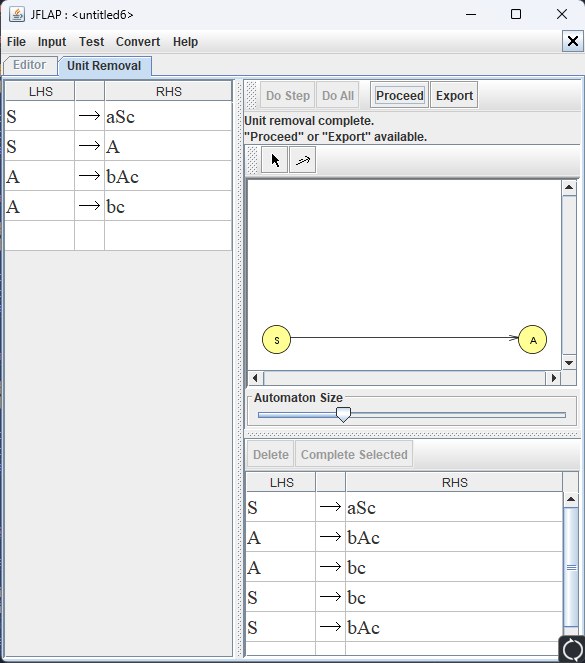
\includegraphics[scale=0.55]{img/grammar_07_simplified.png}
    \caption{Gramática simplificada en JFLAP para el lenguaje $L = \{a^i b^j c^{i+j} \mid i, \ j \geq 1, \ i + j \ par\}$}
    \label{fig:gramatica7_simplified}
  \end{figure}
\end{itemize}

\newpage

% Ejericio 8
\section{Diseñaar una gramática independiente del contexto que genere el lenguaje de las expresiones booleanas con los operadores AND, OR, y NOT, usando paréntesis
para agrupar. Ejemplos: “(true AND false)”, “NOT (true OR false)”, “true AND (false OR true)”.}
\begin{itemize}
  \item \textbf{Explicación de la gramática:} El lenguaje de las expresiones booleanas con los operadores AND, OR, y NOT, usando paréntesis para agrupar, acepta todas las cadenas que siguen la siguiente estructura:
  \begin{itemize}
    \item $S \rightarrow \texttt{true} \mid \texttt{false} \mid \texttt{NOT} \ S \mid S \ \texttt{AND} \ S \mid S \ \texttt{OR} \ S \mid (\ S \ )$
  \end{itemize}
  \item \textbf{Imagen de la gramática en JFLAP:} La gramática diseñada en JFLAP se muestra en la siguiente figura:
  \begin{figure}[H]
    \centering
    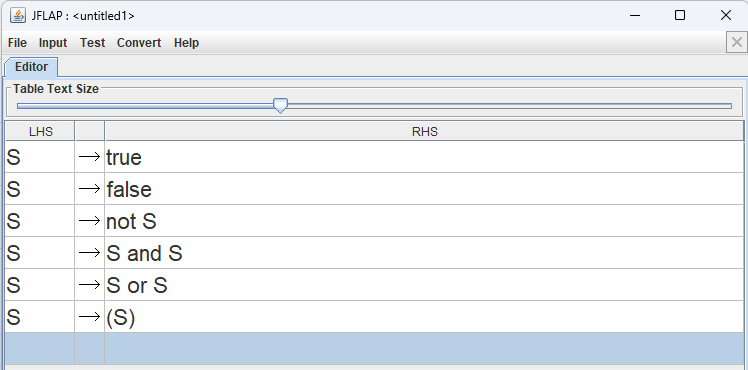
\includegraphics[scale=0.5]{img/grammar_08.png}
    \caption{Gramática diseñada en JFLAP para el lenguaje de las expresiones booleanas con los operadores AND, OR, y NOT, usando paréntesis para agrupar}
  \end{figure}
  \item \textbf{Ejemplos de cadenas generadas:}
  \begin{itemize}
    \item \textbf{Cadena 1:} $(\texttt{true AND false})$
    \begin{itemize}
      \item \textbf{Árbol de análisis sintáctico:} El árbol de análisis sintáctico para la cadena $(\texttt{true AND false})$ se muestra en la siguiente figura:
      \begin{figure}[H]
        \centering
        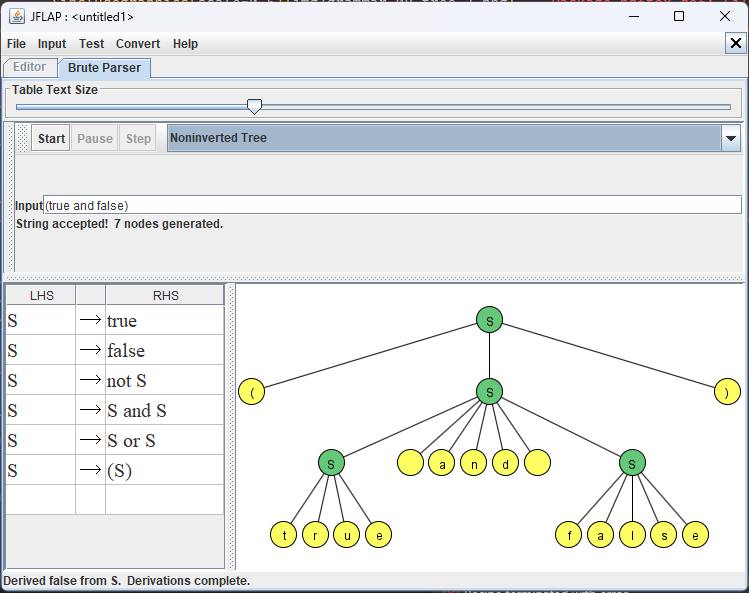
\includegraphics[scale=0.5]{img/grammar_08_tree_1.png}
        \caption{Árbol de análisis sintáctico para la cadena $(\texttt{true AND false})$}
        \label{fig:arbol22}
      \end{figure}
    \end{itemize}
    \item \textbf{Cadena 2:} $\texttt{NOT (true OR false)}$
    \begin{itemize}
      \item \textbf{Árbol de análisis sintáctico:} El árbol de análisis sintáctico para la cadena $\texttt{NOT (true OR false)}$ se muestra en la siguiente figura:
      \begin{figure}[H]
        \centering
        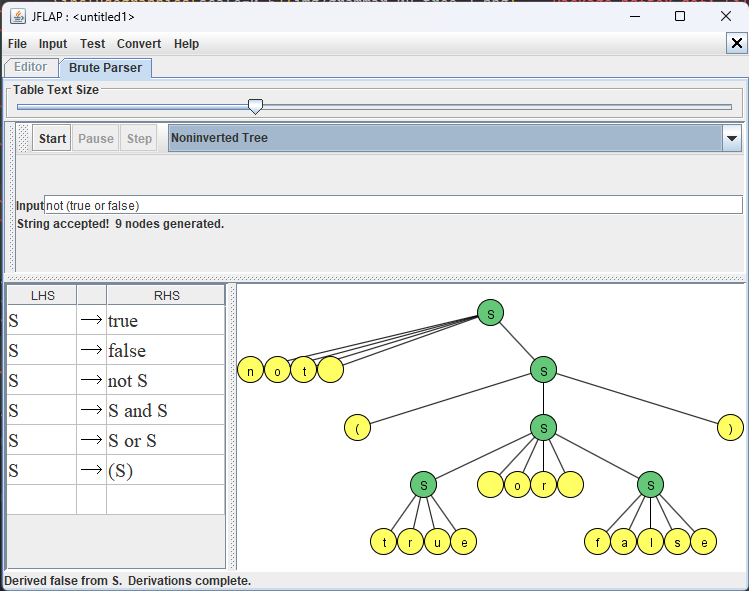
\includegraphics[scale=0.5]{img/grammar_08_tree_2.png}
        \caption{Árbol de análisis sintáctico para la cadena $\texttt{NOT (true OR false)}$}
        \label{fig:arbol23}
      \end{figure}
    \end{itemize}

    \newpage

    \item \textbf{Cadena 3:} $\texttt{true AND (false OR true)}$
    \begin{itemize}
      \item \textbf{Árbol de análisis sintáctico:} El árbol de análisis sintáctico para la cadena $\texttt{true AND}$ $\texttt{(false OR true)}$ se muestra en la siguiente figura:
      \begin{figure}[H]
        \centering
        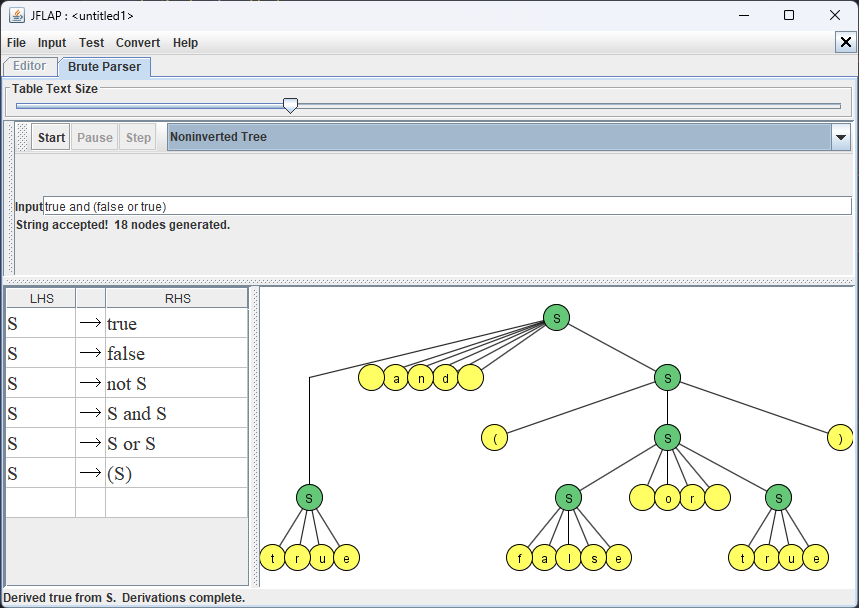
\includegraphics[scale=0.5]{img/grammar_08_tree_3.png}
        \caption{Árbol de análisis sintáctico para la cadena $\texttt{true AND (false OR true)}$}
        \label{fig:arbol24}
      \end{figure}
    \end{itemize}
  \end{itemize}
  % \item \textbf{Imagen de la gramática simplificada en JFLAP:} La gramática simplificada en JFLAP se muestra en la siguiente figura:
  % \begin{figure}[H]
  %   \centering
  %   \includegraphics[scale=0.5]{img/grammar_08_simplified.png}
  %   \caption{Gramática simplificada en JFLAP para el lenguaje de las expresiones booleanas con los operadores AND, OR, y NOT, usando paréntesis para agrupar}
  %   \label{fig:gramatica8_simplified}
  % \end{figure}
\end{itemize}

\newpage

\section{Diseñar una gramática independiente del contexto que genere expresiones aritméticas simples con suma y multiplicación, utilizando los símbolos $+$, $*$, $(, )$ y los números 0, 1, etc. Ejemplos: “1+2”, “(1+2)*3”, “4*(5+6)”.}
\begin{itemize}
  \item \textbf{Explicación de la gramática:} El lenguaje de las expresiones aritméticas simples con suma y multiplicación, utilizando los símbolos $+$, $*$, $(, )$ y los números 0, 1, etc., acepta todas las cadenas que siguen la siguiente estructura:
  \begin{itemize}
    \item $S \rightarrow S + S \mid S * S \mid (S) \mid 0 \mid 1 \mid 2 \mid 3 \mid 4 \mid 5 \mid 6 \mid 7 \mid 8 \mid 9 $
  \end{itemize}
  \item \textbf{Imagen de la gramática en JFLAP:} La gramática diseñada en JFLAP se muestra en la siguiente figura:
  \begin{figure}[H]
    \centering
    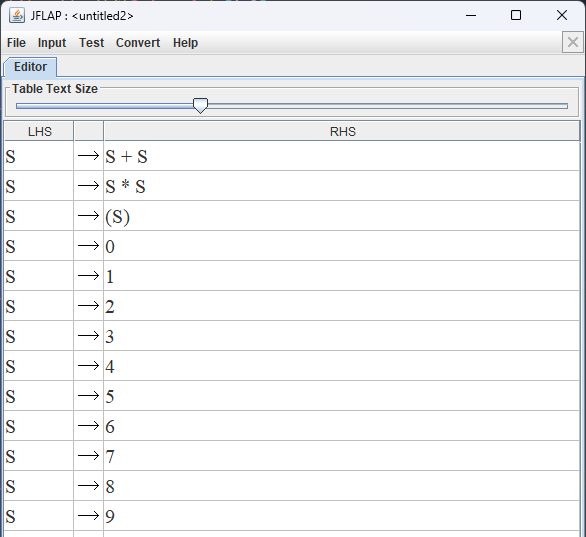
\includegraphics[scale=0.5]{img/grammar_09.png}
    \caption{Gramática diseñada en JFLAP para el lenguaje de las expresiones aritméticas simples con suma y multiplicación}
  \end{figure}

  \newpage

  \item \textbf{Ejemplos de cadenas generadas:}
  \begin{itemize}
    \item \textbf{Cadena 1:} $1+2$
    \begin{itemize}
      \item \textbf{Árbol de análisis sintáctico:} El árbol de análisis sintáctico para la cadena $1+2$ se muestra en la siguiente figura:
      \begin{figure}[H]
        \centering
        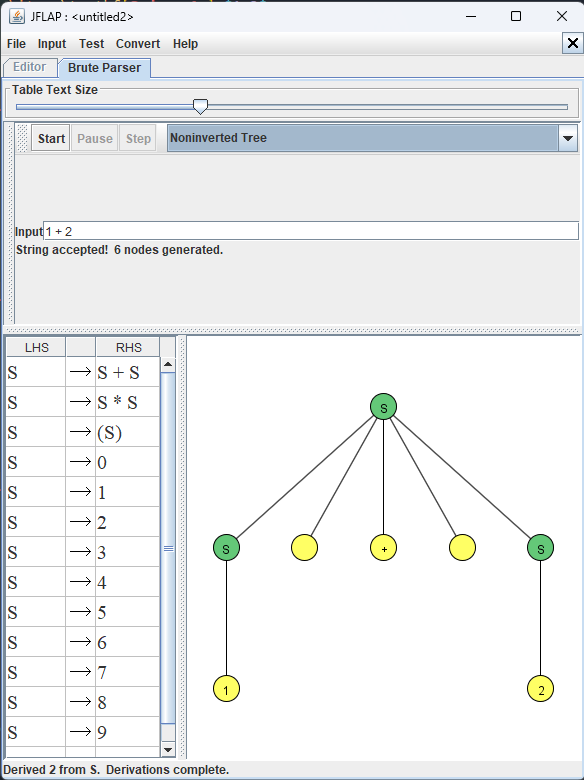
\includegraphics[scale=0.5]{img/grammar_09_tree_1.png}
        \caption{Árbol de análisis sintáctico para la cadena $1+2$}
        \label{fig:arbol25}
      \end{figure}
    \end{itemize}

    \newpage

    \item \textbf{Cadena 2:} $(1+2)*3$
    \begin{itemize}
      \item \textbf{Árbol de análisis sintáctico:} El árbol de análisis sintáctico para la cadena $(1+2)*3$ se muestra en la siguiente figura:
      \begin{figure}[H]
        \centering
        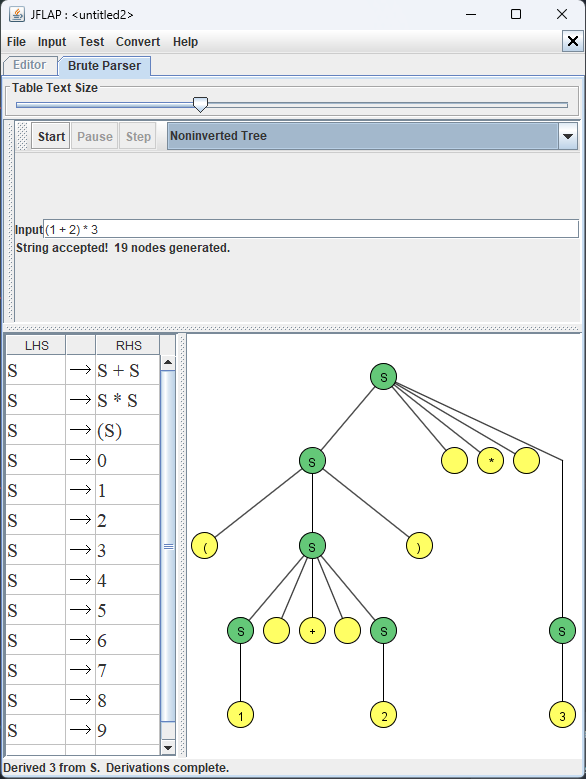
\includegraphics[scale=0.5]{img/grammar_09_tree_2.png}
        \caption{Árbol de análisis sintáctico para la cadena $(1+2)*3$}
        \label{fig:arbol26}
      \end{figure}
    \end{itemize}

    \newpage

    \item \textbf{Cadena 3:} $4*(5+6)$
    \begin{itemize}
      \item \textbf{Árbol de análisis sintáctico:} El árbol de análisis sintáctico para la cadena $4*(5+6)$ se muestra en la siguiente figura:
      \begin{figure}[H]
        \centering
        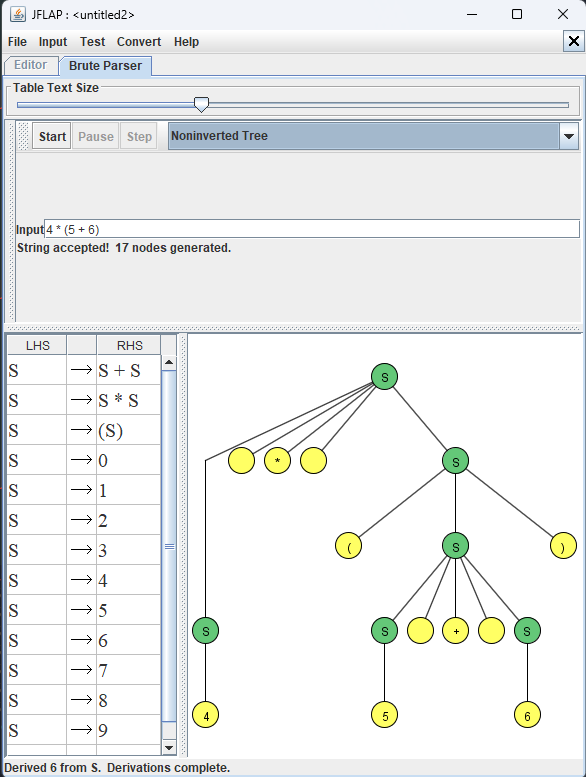
\includegraphics[scale=0.5]{img/grammar_09_tree_3.png}
        \caption{Árbol de análisis sintáctico para la cadena $4*(5+6)$}
        \label{fig:arbol27}
      \end{figure}
    \end{itemize}
  \end{itemize}
  % \item \textbf{Imagen de la gramática simplificada en JFLAP:} La gramática simplificada en JFLAP se muestra en la siguiente figura:
  % \begin{figure}[H]
  %   \centering
  %   \includegraphics[scale=0.5]{img/grammar_09_simplified.png}
  %   \caption{Gramática simplificada en JFLAP para el lenguaje de las expresiones aritméticas simples con suma y multiplicación}
  %   \label{fig:gramatica9_simplified}
  % \end{figure}
\end{itemize}

\newpage

\section{Diseñar una gramática independiente del contexto que genere el lenguaje de listas anidadas usando corchetes, como en los lenguajes de programación. Ejemplos: [], [[]], [[[]]], [[1,2],[3,4]].}
\begin{itemize}
  \item \textbf{Explicación de la gramática:} El lenguaje de listas anidadas usando corchetes, como en los lenguajes de programación, acepta todas las cadenas que siguen la siguiente estructura:
  \begin{itemize}
    \item $S \rightarrow [S] \mid [S, S] \mid \varepsilon$
  \end{itemize}
  \item \textbf{Imagen de la gramática en JFLAP:} La gramática diseñada en JFLAP se muestra en la siguiente figura:
  \begin{figure}[H]
    \centering
    \includegraphics[scale=0.5]{img/grammar_10.png}
    \caption{Gramática diseñada en JFLAP para el lenguaje de listas anidadas usando corchetes}
  \end{figure}
  \item \textbf{Ejemplos de cadenas generadas:}
  \begin{itemize}
    \item \textbf{Cadena 1:} $[]$
    \begin{itemize}
      \item \textbf{Árbol de análisis sintáctico:} El árbol de análisis sintáctico para la cadena $[]$ se muestra en la siguiente figura:
      \begin{figure}[H]
        \centering
        \includegraphics[scale=0.5]{img/grammar_10_tree_1.png}
        \caption{Árbol de análisis sintáctico para la cadena $[]$}
        \label{fig:arbol28}
      \end{figure}
    \end{itemize}

    \newpage

    \item \textbf{Cadena 2:} $[[]]$
    \begin{itemize}
      \item \textbf{Árbol de análisis sintáctico:} El árbol de análisis sintáctico para la cadena $[[]]$ se muestra en la siguiente figura:
      \begin{figure}[H]
        \centering
        \includegraphics[scale=0.5]{img/grammar_10_tree_2.png}
        \caption{Árbol de análisis sintáctico para la cadena $[[]]$}
        \label{fig:arbol29}
      \end{figure}
    \end{itemize}

    \newpage

    \item \textbf{Cadena 3:} $[[[]]]$
    \begin{itemize}
      \item \textbf{Árbol de análisis sintáctico:} El árbol de análisis sintáctico para la cadena $[[[]]]$ se muestra en la siguiente figura:
      \begin{figure}[H]
        \centering
        \includegraphics[scale=0.5]{img/grammar_10_tree_3.png}
        \caption{Árbol de análisis sintáctico para la cadena $[[[]]]$}
        \label{fig:arbol30}
      \end{figure}
    \end{itemize}
  \end{itemize}
  % \item \textbf{Imagen de la gramática simplificada en JFLAP:} La gramática simplificada en JFLAP se muestra en la siguiente figura:
  % \begin{figure}[H]
  %   \centering
  %   \includegraphics[scale=0.5]{img/grammar_10_simplified.png}
  %   \caption{Gramática simplificada en JFLAP para el lenguaje de listas anidadas usando corchetes}
  %   \label{fig:gramatica10_simplified}
  % \end{figure}
\end{itemize}


\end{document}